\documentclass[11pt,a4paper]{amsart}
\usepackage{amsfonts}
\usepackage{physics}
\usepackage{amsthm}
\usepackage{amsmath}
\usepackage{amscd}
\usepackage[latin2]{inputenc}
\usepackage{t1enc}
\usepackage[mathscr]{eucal}
\usepackage{indentfirst}
\usepackage{graphicx}
\usepackage{graphics}
\usepackage{pict2e}
\usepackage{epic}
\numberwithin{equation}{section}
\usepackage[margin=2.9cm]{geometry}
\usepackage{epstopdf}
\usepackage{amsmath,amsthm,verbatim,amssymb,amsfonts,amscd, graphicx}
\usepackage{mathtools}
\usepackage[dvipsnames]{xcolor}
\usepackage{algorithmic}
\usepackage[ruled,vlined]{algorithm2e}

 

\usepackage[backend=biber,date=year,giveninits=true,sorting=nyt,style=alphabetic,natbib=true,maxcitenames=2,maxbibnames=10,url=false,doi=true,backref=false]{biblatex}
\addbibresource{ref.bib}
\renewbibmacro{in:}{\ifentrytype{article}{}{\printtext{\bibstring{in}\intitlepunct}}}
\renewcommand*{\bibfont}{\small}

\DeclareMathOperator{\sgn}{sgn}

\newcommand{\note}[1]{{\leavevmode\color{BrickRed}{#1}}}

 
\usepackage[colorlinks,linkcolor = BrickRed, citecolor=blue]{hyperref} 

 
\definecolor{mypink1}{rgb}{0.858, 0.188, 0.478}
\definecolor{mypink2}{RGB}{219, 48, 122}
\definecolor{mypink3}{cmyk}{0, 0.7808, 0.4429, 0.1412}
\definecolor{mygray}{gray}{0.6}


% For aligned \stackrel, use \leftstackrel
\newlength{\leftstackrelawd}
\newlength{\leftstackrelbwd}
\def\leftstackrel#1#2{\settowidth{\leftstackrelawd}%
{${{}^{#1}}$}\settowidth{\leftstackrelbwd}{$#2$}%
\addtolength{\leftstackrelawd}{-\leftstackrelbwd}%
\leavevmode\ifthenelse{\lengthtest{\leftstackrelawd>0pt}}%
{\kern-.5\leftstackrelawd}{}\mathrel{\mathop{#2}\limits^{#1}}}

 
\theoremstyle{plain}
\newtheorem{Th}{Theorem}
\newtheorem{Lemma}[Th]{Lemma}
\newtheorem{Cor}[Th]{Corollary}
\newtheorem{Prop}[Th]{Proposition}

 \theoremstyle{definition}
\newtheorem{Def}[Th]{Definition}
\newtheorem{Conj}[Th]{Conjecture}
\newtheorem{Rem}[Th]{Remark}
\newtheorem{?}[Th]{Problem}
\newtheorem{Ex}[Th]{Example}

\newcommand{\im}{\operatorname{im}}
\newcommand{\Hom}{{\rm{Hom}}}
\newcommand{\diam}{{\rm{diam}}}
\newcommand{\ovl}{\overline}

\def\R{{\mathbb R}}
\def\Q{{\mathbb Q}}
\def\Z{{\mathbb Z}}
\def\N{{\mathbb N}}
\def\C{{\mathbb C}}
\def\E{{\mathbb E}}
\def\R{{\mathbb R}}
\def\Y{{\mathcal Y}}
\def\L{{\mathcal L}}
\def\H{{\mathcal H}}
\def\D{{\mathcal D}}
\def\P{{\mathbb P}}
\def\M{{\mathbb M}}
\def\V{{\mathcal V}}
\def\d{{\mathsf d}}
\def\A{{\mathbf A}}
\def\x{{\mathbf x}}
\def\b{{\mathbf b}}
\def\a{{\mathbf a}}
\def\Ph{{\mathbf {\Phi}}}

\def\h{{\mathbf{h}}}
\def\G{{\Gamma}}
\def\s{{\sigma}}
\def\e{{\varepsilon}}
\def\l{{\lambda}}
\def\p{{\phi}}
\def\v{{\mathbf{v}}}
\def\t{{\theta}}
\def\z{{\zeta}}
\def\o{{\omega}}
\def\y{{\mathbf{y}}}
\def\g{{\mathbf{g}}}
\def\u{{\mathbf{u}}}
\def\w{{\mathbf{w}}}
\def\var{{\text{Var}}}
\def\ex{{\text{epr}}}
\def\Res{{\text{Res}}}
\def\mse{{\text{MSE}}}



\DeclareMathOperator*{\argmax}{arg\,max}
\DeclareMathOperator*{\argmin}{arg\,min}



\begin{document}
\date{}

\title{Multi-fidelity approximation using bandit learning}
\maketitle

\begin{abstract}
We present a bandit learning approach for multi-fidelity approximation of computationally expensive high-fidelity models. 
Under a linear model assumption, we show that the Linear Regression Monte Carlo (LRMC) estimator for the expected value of the highest fidelity model is consistent as both the budget and exploration round go to infinity. 
Combining the conditional Mean-Squared Error (MSE) estimator and ideas of the UCB algorithm,
we develop a consistent and adaptive model selection procedure which automatically determines the balancing point between exploration and exploitation. 
Under an additional normality assumption on noise, we extend our approach to the case of vector-valued responses with a similar procedure that appropriately captures the correlation structure of the noise between responses. 
As opposed to other methods such as the Multi-fidelity Monte Carlo estimator \cite{Peherstorfer_2016}, our algorithm does not require hierarchical model structure or pre-knowledge on the statistical information of models.  
Numerical experiments are provided in the end to complement our theoretical findings.
\end{abstract}


\tableofcontents

\section{Introduction}

\section{Main results}

\subsection{Linear model assumptions in multi-fidelity models}
In this section, we introduce the Linear Regression Monte Carlo (LRMC) estimators for model selection and estimation in multi-fidelity models. 

Let us first introduce the setup of the problem.
In multi-fidelity models, we assume that the most accurate model is the ground truth.
In practice, it is often impractical to estimate the ground truth directly from the Monte Carlo due to high computational cost. 
Alternatively, people consider using cheaper approximation models (low-fidelity models) to estimate the truth. 
Cheaper models are useful provided they contain information such that if appropriately uncovered, can effectively predict the value of the true model. 
The simplest assumption for such an unknown relationship is a linear model, and this is what we are going to pursue next. 

Let $Y$ be the ground truth, and $X^{(1)}, \cdots, X^{(n)}$ be the $n$ approximation models. 
The cost for obtaining a sample for $Y, X^{(1)}, \cdots, X^{(n)}$ is $c, c_1,\cdots, c_n$, respectively.
$c, c_1, \cdots, c_n$ could be assumed to be random.
For illustration purpose, they are treated as a deterministic non-increasing positive numbers $c\geq c_1\geq\cdots\geq c_n>0$. 

In general, $X^{(1)}, \cdots, X^{(n)}$ may be correlated so that fitting $Y$ using all the possible approximation models can be redundant. 
A more reasonable assumption is to assume that a few of them can be combined to predict $Y$ efficiently.
To formulate the idea,  let $S\subset [n]$ be a selection of approximation models.
Denote the size of $S$ by $s$. 
Suppose $Y$ and $\{X^{(i)}\}_{i\in S}$ satisfy the following linear model assumption:
\begin{align}
Y &= X_S^T\beta_S + \e_S,\label{1},
\end{align}
where $X_S = (X^{(i)})_{i\in S}^T\in\R^{s}$ is the regressor vector, $\beta_S\in\R^{s+1}$ is the coefficient vector and $\e_S\in\R$ is the noise.  
We assume that $\e_S$ is a sub-Gaussian random variable with variance $\sigma_S^2$, i.e., $\|\e_S\|_{\Psi_2}\leq 2$.  
Since our goal is to seek an efficient estimator for $\E[Y]$, taking expectation on both sides of \eqref{1} yields
\begin{align}
\E[Y] = \E[X_S^T]\beta_S.\label{2}
\end{align}
The term $\E[X_S]$ in the right-hand side of \eqref{2} can be estimated by averaging the independent joint samples of $X_S$. 
When $\beta_S$ is known, this is the same as the Monte Carlo applied to the conditional expectation $\E[Y|X_S]$. In this ideal case, what can be gained from sampling from $Y|X_S$ instead of $Y$? 

From a standard calculation, one can check that an $N$-sample Monte Carlo estimator for $\E[Y]$ based on sampling $Y$ has mean-squared error $\var[Y]/N$. The same procedure based on sampling $Y|X_S$, similarly, has mean-squared error $\var[\E[Y|X_S]]/N$. 
Since conditioning does not increase variance, the numerator of the latter is bounded by the numerator of the former for any fixed $N$. 
On the other hand, given a fixed budget, when $\sum_{i\in S}c_i\ll c$, the affordable samples in the latter can be much larger than the former, which can significantly reduce the variance of the estimator.  
Both observations provide some heuristics that \eqref{2} may give rise to a better estimator for $\E[Y]$ under certain circumstances. 
Whereas in practice, neither the true model index set $S$ nor the corresponding $\beta_S$ is known. 
When $\beta_S$ needs to be estimated, the above Monte-Carlo method will no longer be true due to the dependence in the estimator for $\beta_S$. 
Under such circumstance, the problem (under a fixed budget constraint) can be analyzed using a bandit-learning approach, which will be introduced next. 

\begin{table}
  \begin{center}
  \resizebox{\textwidth}{!}{
    \renewcommand{\tabcolsep}{0.4cm}
    \renewcommand{\arraystretch}{1.3}
    {\scriptsize
    \begin{tabular}{@{}cp{0.8\textwidth}@{}}
      $X^{(i)}$ & the $i$-th regressor \\ 
      $Y$ & the response variable (either scalar-valued or vector-valued) \\
      $m$ & the number of samples for exploration\\ 
       $c, c_i$ & the sampling cost of the response variable (high-fidelity model) and the regressors (low-fidelity models)\\
      $B (B_r)$ & the total (remaining) budget\\
      $S$ & the model index set (indices of regressors used in regression)\\
       $N_S$ & the affordable samples in model $S$\\
      $\beta_S$& coefficients (matrix) of model $S$ \\
      $X_{\ex,\ell}$& the $\ell$-th sample in the exploration phase \\
      $Z_S$ & the design matrix in the exploration phase in model $S$ \\
      $x_S$ & the mean of the regressors in model $S$ \\
      $\Sigma_S$& the covariance matrix of the regressors in model $S$ \\
      $\sigma_S^2$ & the variance in model $S$ \\
      $Q$ & the weight matrix in defining the $Q$-weighted risk \\
      $\Gamma_S$ & the covariance matrix of the noise of different response variables \\
    \end{tabular}
  }
    \renewcommand{\arraystretch}{1}
    \renewcommand{\tabcolsep}{12pt}
  }
  \end{center}
  \caption{\small Notation used throughout this article.}\label{tab:notation}
\end{table}


%An $N$-sample Monte Carlo estimator has variance $N^{-1}\var[\sum_{i\in S}\beta_ix_i]$. 
%Under a fixed budget, this can be much cheaper than the Monte Carlo directly applied to $y$, if, for instance, $\var[\sum_{i\in S}\beta_ix_i]\asymp\var[y]$ and $\sum_{i\in S}c_i\ll c$.  
%Whereas the variance of $\sigma_S$ does not seem to play any role. 
%Given a fixed budget, the accuracy of the estimator built in this way could be much better than the Monte Carlo estimator for $y$ if $\sum_{i\in S}c_i\ll c$ since the variance of the estimator is roughly inverse proportional to the sample size.   

\subsection{An idea from bandit learning}

Bandit learning is a powerful tool in sequential decision making.
Its goal is to find a set of actions such that the total regret incurred from it is small in an uncertain environment. 
A comprehensive treatment of the subject can be found in the wonderful book \cite{lattimore2020bandit}.
In our situation, the oracle can be thought as the the ideal situation where $\beta_S$ is known for all $S\subset [n]$. 
In this case, under a fixed budget $B$ and neglecting the floor effect, the `best' model under the linear model assumption is given by the set $S^\star$:
\begin{align}
% \argmin_{S\subset [n]}\frac{\sum_{i\in S}c_i}{B}\var[\E[Y|X_S]] =
S^\star = \argmin_{S\subset [n]}\left(\sum_{i\in S}c_i\right)\var[X_S^T\beta_S].\label{3}
\end{align}
%$S\subset [n]$ can be interpreted as containing intercept or not, as this does not affect the evaluation cost.
Once one knows $S^\star$ and $\beta_{S^\star}$, the optimal estimator for $\E[Y]$ can be built as
\begin{align}
\widehat{\E[Y]}^\star &= \frac{1}{N_{S^\star}}\sum_{j\in [N_S^\star]}X_{{S^\star},j}^T\beta_{S^\star}& N_{S^\star} = \left\lfloor \frac{B}{\sum_{i\in S^\star} c_i}\right\rfloor,\label{4}
\end{align} 
where $X_{{S^\star},j}$'s are iid samples of $X_{S^\star}$. 
When $S^\star$ and $\beta_{S^\star}$ are not known, it would never be optimal to commit all the budget to exploitation. 
In this case, some exploration is needed to learn both $S^\star$ and $\beta_{S^\star}$. 
%We will briefly introduce several variants of approaches in classical stochastic bandits. 
To this end, we will use a variant approach of the Explore-Then-Commit (ETC) in stochastic bandits.

%\subsubsection{Explore-Then-Commit (ETC)}

The Explore-Then-Commit algorithm \cite[Chapter 6]{lattimore2020bandit} divides the budget into two parts: one for exploration and the other for exploitation. 
In our case, this suffices to first use a portion of the budget to learn different models $X_S$, then spend the rest of the budget using the optimal model identified in exploration to build the estimator. 
%To formulate the idea, we shall introduce a few notations. 

Let $m\in\N$ be the number of samples used in the exploration stage. 
Since we have no clue of the best regression model,  it is necessary to draw complete samples consisting of both $Y$ and $X^{(i)}$, $i\in [n]$. 
Denote each sample by $X_{\ex, \ell}$, where $\ell\in [m]$.
$X_{\ex,i}|_S$ and $X_{\ex,i}|_Y$ are the restriction of $X_{\ex,i}$ to the model $X_S$ and $Y$, respectively.  
In this case, $\beta_S$ can be estimated by the least squares, 
\begin{align}
&\widehat{\beta}_S= (Z_S^TZ_S)^{-1}Z_S^TX_\ex|_Y& Z_S = (X_{\ex, 1}|_S, \cdots, X_{\ex, m}|_S)^T.
\end{align} 
The total cost for exploration is $m(c+\sum_{i\in [n]}c_i)$, and the remaining budget for exploitation is $B_r:=B -m(c+\sum_{i\in [n]}c_i)$.
For model $X_S$, let $x_S$ and $\Sigma_S$ denote its mean and covariance matrix, respectively. 
The affordable samples which can be drawn from $X_S$ is $N_S = \lfloor B_r/\sum_{i\in S}c_i\rfloor$. 
To make analysis simpler, we will not reuse samples in the exploration stage for exploitation purpose.  
The LRMC estimator associated with model $X_S$ is 
\begin{align}
\widehat{\E[Y]}_S = \frac{1}{N_S}\sum_{i\in [N_S]}X_{S,i}^T\widehat{\beta}_S.\label{LRMC}
\end{align}
%In other words, the estimator is built only based on the samples drawn under the remaining budget.    
The next theorem states that $\widehat{\E[Y]}_S$, as an estimator for $\E[Y]$, is consistent as both $m, N_S\to\infty$. 
\begin{Th}[Consistency of LRMC]\label{thm:cons}
Assume $\|X_S\|\leq K^2(\E[\|X_S\|^2])^{1/2}$ for some $K>0$.
Assume also that $\Lambda_S := x_Sx_S^T+\Sigma_S$ is invertible. 
Consider the LRMC estimator $\widehat{\E[Y]}_S$ defined in \eqref{LRMC} as an estimator for $\E[Y]$. 
Denote the conditional mean-squared error of $\widehat{\E[Y]}_S$ on $\widehat{\beta}_S$ as $\mse_S|_{\widehat{\beta}_S}$. 
Then, the following consistency result holds:
%\begin{itemize}
%\item If $x_S=0$, then $$\mse_S|_{\widehat{\beta}_S} = \frac{\widehat{\beta}_S^T\Sigma_S\widehat{\beta}_S}{N_S}$$
%\item If $x_S\neq 0$, then with probability at least $1-1/m^2$,  $$\mse_S|_{\widehat{\beta}_S} = \mathcal O\left(\frac{\widehat{\beta}_S^T\Sigma_S\widehat{\beta}_S}{N_S}+\sigma_S^2x_S^T\Lambda_S^{-1}x_S\frac{\log m}{m}\right).$$
%\end{itemize}
\begin{align}
&\mse_S|_{\widehat{\beta}_S} = \mathcal O\left(\frac{\widehat{\beta}_S^T\Sigma_S\widehat{\beta}_S}{N_S}+\sigma_S^2x_S^T\Lambda_S^{-1}x_S\frac{\log m}{m}\right)&m, N_S\to\infty\label{sd}
\end{align}
\end{Th}

\begin{Rem}
When $x_S =0$, the second term on the right-hand side of \eqref{sd} disappeared so the conditional mean-squared error is consistent for every fixed $m$. 
In general, $x_S^T\Lambda_S^{-1}x_S = \tr(\Lambda_S^{-1}x_Sx_S^T)\leq \tr(\Lambda_S^{-1}(x_Sx_S^T+\Sigma_S))= s$. Plugging this into \eqref{sd} yields $\mse_S|_{\widehat{\beta}_S} = \mathcal O\left(\frac{\widehat{\beta}_S^T\Sigma_S\widehat{\beta}_S}{N_S}+s\sigma_S^2\frac{\log m}{m}\right)$.
\end{Rem}




\begin{proof}[Proof of Theorem~\ref{thm:cons}]
Conditional on $\widehat{\beta}_S$, $\widehat{\E[Y]}_S$ is the Monte-Carlo estimator for $x^T_S\widehat{\beta}_S$. By the bias-variance decomposition, 
\begin{align}
\E\left[(\widehat{\E[Y]}_S-\E[Y])^2\big |\widehat{\beta}_S\right] &= \var\left[\widehat{\E[Y]}_S\big |\widehat{\beta}_S\right] + (x_S^T(\widehat{\beta}_S-\beta_S))^2\nonumber\\
& = \frac{1}{N_S}\tr(\Sigma_S\widehat{\beta}_S\widehat{\beta}_S^T) + (\widehat{\beta}_S-\beta_S)^Tx_Sx_S^T(\widehat{\beta}_S-\beta_S).\label{ana}
\end{align} 
%When $x_S=0$, the second term in \eqref{ana} vanishes and the desired result follows immediately.  
We need to bound the second term in \eqref{ana}.
Note that  
\begin{align}
\widehat{\beta}_S - \beta_S =  (Z_S^TZ_S)^{-1}Z_S^T\eta_S = Z_S^\dagger\eta_S,\label{pt}
\end{align}
where $\eta_S/\sigma_S\in\R^m$ is an isotropic sub-Gaussian random vector, i.e., $\E[\eta_S\eta_S^T] = \sigma_S^2I_m$. Therefore,
\begin{align}
&(\widehat{\beta}_S-\beta_S)^Tx_Sx_S^T(\widehat{\beta}_S-\beta_S) = \|B_S\eta_S\|^2&B_S = \sqrt{x_Sx_S^T}Z_S^\dagger.\label{exp1}
\end{align}
Conditional on $X_{\ex,\ell}|_S, \ell\in [m]$, we can apply the Hanson-Wright inequality \cite[Theorem 6.3.2]{Vershynin_2018} to \eqref{exp1} to obtain 
\begin{align*}
\P\left(\left|\|B_S\eta_S\|-\sigma_S\|B_S\|_F\right|>\sigma_St\right)\leq 2\exp(-ct^2/\|B_S\|_2^2),
\end{align*}
where $c$ is an absolute constant. 
Setting $t=k\|B_S\|_F$ and noting $\|B_S\|_F = \|B_S\|_2= \|(Z_S^\dagger)^T x_S\|$, 
\begin{align}
\|B_S\eta_S\|^2\leq \sigma^2_S(k+1)^2\|(Z_S^\dagger)^T x_S\|^2\label{oi}
\end{align}
holds with probability at least $1-2\exp(-ck^2)$. 
On the other hand, 
\begin{align}
\|(Z_S^\dagger)^T x_S\|^2 = \tr((Z_S^TZ_S)^{-1} x_Sx_S^T) = \frac{1}{m}\tr(\left(\frac{1}{m}Z_S^TZ_S\right)^{-1} x_Sx_S^T).\label{bdd}
\end{align}
Using the results in covariance estimation, with probability at least $1-1/2m^2$,
\begin{align}
&\left\|\frac{1}{m}Z_S^TZ_S -\Lambda_S\right\|_2\leq CK\sqrt{\frac{s\log (sm)}{m}}\|\Lambda_S\|_2,\label{cov}
\end{align}
where $C$ is an absolute constant. 
Note for an invertible matrix $A$ and perturbation $\Delta A$, the perturbed inverse $(A+\Delta A)^{-1}$ satisfies
$$(A+\Delta A)^{-1} =  A^{-1}-A^{-1}\Delta AA^{-1} + \text{high order terms}.$$ 
This combined with \eqref{cov} yields that with probability at least $1-1/2m^{2}$,
\begin{align}
&\left(\frac{1}{m}Z_S^TZ_S\right)^{-1} = \Lambda_S^{-1} + E_S& \|E_S\|_2\leq \frac{CK}{\sigma^2_{\min}(\Lambda_S)}\sqrt{\frac{s\log (sm)}{m}}\|\Lambda_S\|_2,
\end{align}
which immediately implies that
%\begin{align*}
%\frac{1}{m}\tr(\left(\frac{1}{m}Z_S^TZ_S\right)^{-1} x_Sx_S^T) &= \frac{1}{m}\tr((\Lambda_S^{-1} + E_S) x_Sx_S^T)\\
%&\leq \frac{1}{m}\tr((\Lambda_S^{-1} + e_SI_m) x_Sx_S^T),\\
%\frac{1}{m}\tr(\left(\frac{1}{m}Z_S^TZ_S\right)^{-1} x_Sx_S^T) &= \frac{1}{m}\tr((\Lambda_S^{-1} + E_S) x_Sx_S^T)\\
%&\geq \frac{1}{m}\tr((\Lambda_S^{-1} - e_SI_m) x_Sx_S^T).
%\end{align*}
\begin{align}
\left|\tr(\left(\frac{1}{m}Z_S^TZ_S\right)^{-1} x_Sx_S^T)\right|\leq x_S^T\Lambda_S^{-1}x_S +\frac{CK}{\sigma^2_{\min}(\Lambda_S)}\sqrt{\frac{s\log (sm)}{m}}\|\Lambda_S\|_2\|x_S\|^2. \label{lk}
\end{align}
%These together with \eqref{bdd} yield that with probability $1-1/2m^2$, $\|Z_S^\dagger x_S\|^2 = \mathcal O (1/m)$.
Putting \eqref{lk}, \eqref{bdd}, \eqref{oi}, \eqref{exp1} and \eqref{ana} together and taking $k=C'\sqrt{\log m}$ with $C'$ chosen sufficiently large finishes the proof. 
\end{proof}



Note that \eqref{ana} provides a formula for the conditional mean-squared error of $\widehat{\E[Y]}_S$ for different models $X_S$. 
It is tempting to select the model with the least mean-squared error for exploitation. 
Nevertheless, quantities such as $\Sigma_S, x_S$ and $(\widehat{\beta}_S-\beta_S)$ in \eqref{ana} are unknown, and this makes \eqref{ana} of little practical use in general. 
A possible way to get around this is to replace them with appropriate estimates in the exploration. 
For example, $x_S$ and $\Sigma_S$ can be computed using their sample estimators:
\begin{align}
\widehat{x}_S &= \frac{1}{m}\sum_{\ell\in [m]}X_{\ex, \ell}|_S\nonumber\\
\widehat{\Sigma}_S &= \frac{1}{m-1}\sum_{\ell\in [m]}(X_{\ex, \ell}|_S-\widehat{x}_S)(X_{\ex, \ell}|_S-\widehat{x}_S)^T.\label{e1}
\end{align} 
On the other hand, we can approximate $(\widehat{\beta}_S-\beta_S)^Tx_Sx_S^T(\widehat{\beta}_S-\beta_S)$ by its conditional expectation on $Z_S$, 
\begin{align}
(\widehat{\beta}_S-\beta_S)^Tx_Sx_S^T(\widehat{\beta}_S-\beta_S)&\approx \E\left[(\widehat{\beta}_S-\beta_S)^Tx_Sx_S^T(\widehat{\beta}_S-\beta_S)\big | Z_S\right]\nonumber\\
& = \sigma_S^2\tr(x_Sx_S^T(Z_S^TZ_S)^{-1})\nonumber\\
& \approx \widehat{\sigma}_S^2\tr(\widehat{x}_S\widehat{x}_S^T(Z_S^TZ_S)^{-1}),\label{sec}
\end{align}
where $\widehat{\sigma}^2_S$ is the model variance estimator from the exploration stage:
\begin{align}
\widehat{\sigma}^2_S = \frac{1}{m-|S|}\sum_{\ell\in [m]}\left(X_{\ex,\ell}|_Y -X_{\ex,\ell}|_S\widehat{\beta}_S \right)^2. 
\end{align}
An alternative method to compute $(\widehat{\beta}_S-\beta_S)^Tx_Sx_S^T(\widehat{\beta}_S-\beta_S)$ is to use a highly-confident upper bound. 
Given $\delta_m$ where $\delta_m\to 0$ as $m\to\infty$, one can use the sub-Gaussian assumption to obtain a $(1-\delta_m)$-confidence set $C(S,\delta_m)$ for $\beta_S$: 
\begin{align}
\P\left(\beta_S-\widehat{\beta}_S\in C(S,\delta_m) \big | Z_S\right)\geq 1-\delta_m.\label{e3}
\end{align}
Such $C(S,\delta_m)$ can be constructed based on the Hanson-Wright inequality,
\begin{align}
\P\left(\left|\|(Z_S^TZ_S)(\widehat{\beta}_S-\beta_S)\| -\sigma_S\|Z^T_S\|_F\right|>\sigma_St\right) &= \P\left(\left|\|Z^T_S\eta_S\| -\sigma_S\|Z^T_S\|_F\right|>\sigma_St\right)\nonumber\\
&\leq 2\exp(-ct^2/\|Z^T_S\|^2_2).\label{212}
\end{align}
Taking $t = \|Z^T_S\|_2\sqrt{\log(2/\delta_m)/c}$ and replacing $\sigma_S$ by $\widehat{\sigma}_S$ yields an approximate $C(S,\delta_m)$:
\begin{align}
C(S,\delta_m) = \left\{z: \left|\|(Z_S^TZ_S)z\| -\widehat{\sigma}_S\|Z^T_S\|_F\right|>\widehat{\sigma}_S \|Z^T_S\|_2\sqrt{\log(2/\delta_m)/c}\right\}.\label{213}
\end{align}
Then with probability at least $1-\delta_m$, 
\begin{align}
(\widehat{\beta}_S-\beta_S)^Tx_Sx_S^T(\widehat{\beta}_S-\beta_S)\leq \sup_{y\in C(S,\delta_m)}(y^Tx_S)^2\approx \sup_{y\in C(S,\delta_m)}(y^T\widehat{x}_S)^2.  \label{usef}
\end{align}
Plugging \eqref{e1}, \eqref{sec} and \eqref{e3} into \eqref{ana} yields the following estimators for $\mse_S|_{\widehat{\beta}_S}$:
\begin{align}
\widehat{\mse}_S|_{\widehat{\beta}_S} = \frac{1}{N_S}\widehat{\beta}_S^T\widehat{\Sigma}_S\widehat{\beta}_S + \widehat{\sigma}_S^2\widehat{x}_S^T(Z_S^TZ_S)^{-1}\widehat{x}_S\label{001}
\end{align}
or
\begin{align}
\widehat{\mse}_S|_{\widehat{\beta}_S} = \frac{1}{N_S}\widehat{\beta}_S^T\widehat{\Sigma}_S\widehat{\beta}_S + \sup_{y\in C(S,\delta_m)}(y^T\widehat{x}_S)^2.\label{002}
\end{align}

By comparing the estimated conditional mean-squared error $\widehat{\mse}_S|_{\widehat{\beta}_S}$, one can decide which model to use for the Monte-Carlo estimator in the exploitation. 
However, this idea is only valid under assumption \eqref{1}. 
One can check the model validity using the \texttt{p}-values of the estimated coefficients. 
This corresponds to testing the hypothesis $\beta_S=0$ under a given significance level $\delta>0$.  
The test statistics can be derived using \eqref{213}:
%For every $i\in S$, under the null hypothesis $\beta_S= 0$, 
%\begin{align}
%(Z_S^TZ_S)\widehat{\beta}_S = Z^T_S\eta_S.
%\end{align} 
%By the Hanson--Wright inequality, 
%\begin{align}
%\P\left(\left|\|(Z_S^TZ_S)\widehat{\beta}_S\| -\sigma_S\|Z^T_S\|_F\right|>\sigma_St\right) &= \P\left(\left|\|Z^T_S\eta_S\| -\sigma_S\|Z^T_S\|_F\right|>\sigma_St\right)\nonumber\\
%&\leq 2\exp(-ct^2/\|Z^T_S\|^2_2),
%\end{align} 
%where $c$ is an absolute constant. 
%Taking $t = \|Z^T_S\|_2\sqrt{\log(2/\delta)/c}$ and replacing $\sigma_S$ by $\widehat{\sigma}_S$ yields the following test statistic:
\begin{align}
T_{S}(\delta) = \mathbb I\left(\left|\|(Z_S^TZ_S)\widehat{\beta}_S\| -\widehat{\sigma}_S\|Z^T_S\|_F\right|>\widehat{\sigma}_S \|Z^T_S\|_2\sqrt{\log(2/\delta)/c}\right).
\end{align}
where $T_S>0$ means the linear model assumption is valid.
One can also use the Bonferroni bound to construct $T_S$ by assigning \texttt{p}-values $w_i\delta$ to $i\in S$ such that $\sum_{i\in [S]}w_i = 1$. 
When $\eta_S$ is Gaussian, the distribution of the both test statistics are explicitly known, and one can compute the corresponding tail probability instead of using concentration inequalities. 
Combining the ideas above we have the following Explore-Then-Commit LRMC (ETC-LRMC) algorithm.
%Before giving the details, we make two comments. 
%Firstly, for a fixed regression model $X_S$, we will consider both models with and without intercept, since they have the same computational cost. 
%Secondly, an exhaustive search for all subsets $S\subset [n]$ can be expensive when $n$ is reasonably large. 
%Also, if all model variances are low, then a complete selection procedure will tend to be biased towards choosing single-variate models.  
%To fix these issues, we will choose an extra parameter $k\leq n$ determining the size of the model. 

\medskip

\begin{algorithm}[H]
 \KwIn{$B$: total budget \\
 \ \ \ \ \ \ \ \ \ \ $m$: exploration sample size\\
 \ \ \ \ \ \ \ \ \ \  $c, c_i$: cost parameters\\
 \ \ \ \ \ \ \ \ \ \  $\delta$: significance parameter\\}
 \KwOut{An LRMC estimator for the expectation of the ground truth}
 \begin{algorithmic}[1]
 \STATE{collect $m$ joint samples of $(Y, X_1,\cdots, X_n)$}
 \STATE{compute the remaining budget $B_r = B-m(c+\sum_{i\in [n]}c_i)$}
 \FOR{$S\subset [n]$ (with/without the intercept)}
 \STATE{compute the least-squares estimate $\widehat{\beta}_S$ for model $X_S$}
 \STATE{compute the test statistic $T_S(\delta)$}
 \IF{$T_S(\delta)>0$}
% \STATE{compute the sample covariance matrix $\widehat{\Sigma}_S$ and the estimated model variance $\widehat{\sigma}^2_S$}
 \STATE{compute $\widehat{\mse}_S|_{\widehat{\beta}_S}$ using \eqref{001} or \eqref{002}}
 \ELSE
 \STATE{set $\widehat{\mse}_S|_{\widehat{\beta}_S} = \infty$}
 \ENDIF
 \ENDFOR
\STATE{select $S^\star = \argmin_{S}\widehat{\mse}_S|_{\widehat{\beta}_S}$}
\STATE{return $\widehat{\E[Y]}_{S^\star}$}
 \end{algorithmic}
\caption{Explore-Then-Commit LRMC (ETC-LRMC)} 
\label{alg:ETC}
\end{algorithm}

\subsection{An adaptive Explore-Then-Commit LRMC algorithm}

Similar to the Explore-Then-Commit algorithm in bandit learning, Algorithm \ref{alg:ETC} requires $m$ as an input. 
Since $m$ plays a crucial role in balancing the exploration and exploitation, an arbitrary choice of it may result in underperformance of the algorithm. 
Whereas choosing the optimal $m$ is often difficult in practice. 
In our setup, we propose a possible way to determine $m$ in an adaptive manner.  

We will use \eqref{001} as our estimate for the conditional mean-squared error for model $X_S$:
\begin{align}
\widehat{\mse}_S|_{\widehat{\beta}_S} = \frac{1}{N_S}\widehat{\beta}_S^T\widehat{\Sigma}_S\widehat{\beta}_S + \widehat{\sigma}_S^2\widehat{x}_S^T(Z_S^TZ_S)^{-1}\widehat{x}_S.\label{214}
\end{align}
The right-hand side of \eqref{214} consists of two parts of errors. The first part is the variance of the estimator which decays as $1/N_S$. 
%When $N_S$ is large, $\frac{1}{N_S}\widehat{\beta}_S^T\widehat{\Sigma}_S\widehat{\beta}_S$ and $\frac{1}{N_S}{\beta}_S^T\Sigma_S\widehat{\beta}_S$ are approximately at the same order. 
The second part stems from estimating $\beta_S$ in the exploration phase, which decays as $\mathcal\sigma^2_S\log m/m$ and is independent of the budget. 

Suppose the budget is sufficiently large. 
When $m$ is small, the second term in \eqref{214} will likely dominate. 
In this case, it would be wasteful to keep increasing $N_S$ if the first term in \eqref{214} has already reduced to the same order as the second term before the remaining budget is used up. 
In this case, more exploration will help decrease the mean-squared error of the estimator. 
One can use this process to push up $m$ one step at a time until the balancing point occurs. 

For implementation, fixed $m$ and model $X_S$.
One can compute both terms on the right-hand of \eqref{214} using the exploration data.
If the first term is greater than the second term, then it implies that current exploration is sufficient so one can devote all the remaining budget for exploitation.  
On the other hand, if the first term is less than the second term, one can increase $m$ to $m+1$ and recompute the value of the first term. 
Note that this step is purely theoretical and does not require taking additional samples in practice. 
If the recomputed value is below the second term, then the current exploration may not be sufficient so one can increase the exploration round from $m$ to $m+1$. 
Otherwise $m$ (or $m+1$) is the balancing point between the exploration and the exploitation. 

In applications, $N_S$ is sufficiently large throughout the exploration phase. 
This ensures that $\widehat{\beta}_S^T\widehat{\Sigma}_S\widehat{\beta}_S/N_S$ and $\widehat{\beta}_S^T\Sigma_S\widehat{\beta}_S/N_S$ are approximately at the same order despite the error incurred in the estimation of $\Sigma_S$. 
On the other hand, $m$ usually starts from some small number, i.e., the same order as the number of the regressors, estimation error of the second term in \eqref{214} is often not negligible at the beginning stage.  
Under such circumstance, we may use the trick of taking upper confidence bound to encourage exploration.
The bonus brought by the upper confidence bound diminishes to zero as exploration rounds become larger. 
This is similar to the Upper Confidence Bound (UCB) algorithm \cite{auer2002finite} in stochastic bandits. 

To illustrate how this works let us assume that the noise is Gaussian. 
It follows from Cochran's theorem that 
\begin{align}
\frac{(m-s)\widehat{\sigma}^2_S}{\sigma^2_S}\sim\chi^2_{m-s},
\end{align}
where $\chi^2_{m-s}$ is the chi-squared distribution with degree of freedom $m-s$. 
Denote $F_{m-s}^{-1}$ as the inverse cumulative distribution function of $\chi^2_{m-s}$. Then, it is easy to check that for any $\alpha>0$, 
\begin{align}
\P\left(\sigma_S^2\leq \frac{m-s}{F^{-1}_{m-s}(\alpha)}\widehat{\sigma}^2_S\right) = 1-\alpha. \label{chi}
\end{align}
This gives an upper confidence bound for the model variance using its estimate. 
Putting the above ideas together we arrive at the following adaptive version of the Algorithm \ref{alg:ETC}:

\medskip

\begin{algorithm}[H]
 \KwIn{$B$: total budget \\
 \ \ \ \ \ \ \ \ \ \  $c, c_i$: cost parameters\\
 \ \ \ \ \ \ \ \ \ \  $\delta$: significance parameter\\
 \ \ \ \ \ \ \ \ \ \  $\alpha_t$: UBC paramters}
 \KwOut{An LRMC estimator for the expectation of the ground truth}
 \begin{algorithmic}[1]
 \STATE set the initial exploration round $m=n+2$
 \STATE compute the maximum exploration round $M = \lfloor B/(c+\sum_{i\in [n]}c_i)\rfloor$
 \WHILE{$m< M$}
 \STATE Use the Explore-Then-Commit algorithm to find the best model $S^\star$, and $s^\star = |S^\star|$
 \STATE For model $X_{S^\star}$, compute the next-step variance error $E_1 = \widehat{\beta}_{S^\star}^T\widehat{\Sigma}_{S^\star}\widehat{\beta}_{S^\star}/\tilde{N}_{S^\star}$, where $\tilde{N}_{S^\star}$ is the number of affordable samples when $m+1$ rounds of exploration are taken, and the estimation error $E_2 = \widehat{\sigma}_{S^\star}^2\widehat{x}_{S^\star}^T(Z_{S^\star}^TZ_{S^\star})^{-1}\widehat{x}_{S^\star}$
\IF{$E_1<\frac{m-s^\star}{F^{-1}_{m-s^\star}(\alpha_m)}E_2$}
        \STATE $m = m + 1$
    \ELSE
        \STATE $m = M$
     \ENDIF
 \ENDWHILE
\STATE{return $\widehat{\E[Y]}_{S^\star}$}
 \end{algorithmic}
\caption{Adaptive Explore-Then-Commit LRMC} 
\label{alg:aETC}
\end{algorithm}

For the step $5$ and $6$ in Algorithm \ref{alg:aETC}, we used the precise upper confidence bound for $\sigma_S^2$ when the noise is Gaussian. 
For general sub-Gaussian noises, one can `formally' use the Bernstein inequality for sum of iid sub-exponential random variables to derive the upper confidence bound instead. The details are similar to \eqref{212} and \eqref{213}, hence are not derived here. 

Note that for fixed $S$, Algorithm \ref{alg:aETC} ensures that both $m$ and $N_S$ go to infinity as $B\to\infty$, since otherwise $m$ will be bounded, and the second term in \eqref{214} will dominate so that Algorithm \ref{alg:aETC} will force $m$ to increase. This observation combined with Theorem \ref{thm:cons} implies that the consistency of the Adaptive Explore-Then-Commit LRMC estimator. 

\begin{Th}[Consistency of the adaptive ETC-LRMC]
The Adaptive Explore-Then-Commit LRMC estimator is consistent as budget goes to infinity. 
\end{Th} 
\begin{proof}
The adaptive ETC-LRMC algorithm guarantees that $m\to\infty$ as $B\to\infty$. For sufficiently large $m$, 
\begin{align*}
 \frac{1}{N_S}\widehat{\beta}_S^T\widehat{\Sigma}_S\widehat{\beta}_S \approx  \frac{1}{N_S}\beta_S^T\Sigma_S\beta_S  \approx \frac{1}{B-(c+\sum_{i\in S}c_i)m}\beta_S^T\Sigma_S\beta_S\\
  \widehat{\sigma}_S^2\widehat{x}_S^T(Z_S^TZ_S)^{-1}\widehat{x}_S\approx \frac{1}{m}\sigma_S^2x_S^T\Lambda_S^{-1}x_S \approx \frac{1}{m}\sigma_S^2x_S^T\Lambda_S^{-1}x_S.
\end{align*}
Two terms are equal if $m$ equals 
\begin{align*}
m_S^* = \frac{B\sigma_S^2x_S^T\Lambda_S^{-1}x_S}{(c+\sum_{i\in S}c_i)\sigma_S^2x_S^T\Lambda_S^{-1}x_S+\beta_S^T\Sigma_S\beta_S}.
\end{align*}
Thus, for sufficiently large $B$, the model finally chosen by the adaptive ETC-LRMC algorithm belongs to
\begin{align*}
\argmin_{S\subset [n]}\frac{1}{B-(c+\sum_{i\in S}c_i)m_S^*}\beta_S^T\Sigma_S\beta_S+ \frac{1}{m^*}\sigma_S^2x_S^T\Lambda_S^{-1}x_S.
\end{align*}
However, for a fixed model, the LRMC estimator is consistent as $m, N_S\to\infty$ according to Theorem \ref{thm:cons}. The proof is complete.  
\end{proof}


\subsection{Vector-valued responses}

Results in previous sections can be generalized to the case of multiple response regression.
Let $Y = (Y^{(1)}, \cdots, Y^{(p)})^T\in\R^p$ be a $p$-dimensional response vector.
The linear regression assumption in \eqref{1} is modified as follows:
\begin{align}
&Y^{(t)} = X_S^T\beta_{S, t} + \e_{S, t}& t = 1, \cdots, p. \label{newass}
\end{align}
where $\e_S = (\e_{S, 1}, \cdots, \e_{S, p})\sim\mathcal N (0, \Gamma_S)$. 
Here we strengthen the noise assumption which will help us better capture some low-dimensional structure. 
To generalize the mean-squared error to vector-valued estimation, we consider a common class of risk functionals called $Q$-weighted risk which is defined as follows. 
Let $Q\in\R^{d\times s}$ and $\widehat{\theta}_n$ be an estimator for $\theta\in\R^s$. 
The \emph{$Q$-weighted risk} of $\widehat{\theta}_n$ is defined as 
\begin{align}
R_Q(\widehat{\theta}_n) = \E\left[\|Q(\widehat{\theta}_n-\theta)\|^2\right] = \E\left[(\widehat{\theta}_n-\theta)^TQ^TQ(\widehat{\theta}_n-\theta)\right].
\end{align}

By a similar argument as the proof of Theorem \ref{thm:cons}, we can obtain the consistency of the LRMC when $Y$ is a vector-valued response under the $Q$-weighted risk:  


\begin{Th}[Consistency of LRMC with vector-valued response]\label{thm:consv}
Let $Y = (Y^{(1)}, \cdots, Y^{(p)})^T\in\R^p$ be a multi-dimensional response vector.
Under the same conditions as in Theorem \ref{thm:cons} and \eqref{newass},
the following consistency result holds under the $Q$-weighted risk:
\begin{align}
&R_Q(\widehat{\E[Y]}_S)|_{\widehat{\beta}_S} \lesssim \frac{1}{N_S}\tr(\Sigma_S\widehat{\beta}_S^TQ^TQ\widehat{\beta}_S) + \tr(Q\Gamma_SQ^T)x_S^T\Lambda_S^{-1}x_S\frac{\log m}{m}.&m, N_S\to\infty\label{sd}
\end{align}
\end{Th}
\begin{proof}
Adopting the same notation as before, and defining $\beta_S = (\beta_{S,1}, \cdots, \beta_{S,p})^T$, we can employ a similar computation as before that the conditional $Q$-weighted risk of the LRMC on $\widehat{\beta}_S$ is 
\begin{align}
R_Q(\widehat{\E[Y]}_S)|_{\widehat{\beta}_S} = \frac{1}{N_S}\tr(\Sigma_S\widehat{\beta}_S^TQ^TQ\widehat{\beta}_S) + x_S^T(\widehat{\beta}_S-\beta_S)^TQ^TQ(\widehat{\beta}_S-\beta_S)x_S.
\end{align}
Conditional on $X_{\ex,\ell}|_S, \ell\in [m]$,
\begin{align}
Q(\widehat{\beta}_S-\beta_S) = Q(\eta_{S,1}, \cdots, \eta_{S, m})(Z_S^\dagger)^T,
\end{align}
where $\eta_{S,\ell}\sim\mathcal N(0,\Gamma_S)$ are iid random vectors. 
Let $r_S = \rank(\Gamma_S)$.
By properties of multivariate normal distributions, there exists a $P_S\in\R^{p\times r_S}$ such that $\eta_{S,\ell} = P_S\xi_{S, \ell}$, where $\xi_{S,\ell}$ are iid $r_S$-dimensional normal distributions, and $P_SP_S^T = \Gamma_S$. 
Thus, 
\begin{align}
&x_S^T(\widehat{\beta}_S-\beta_S)^TQ^TQ(\widehat{\beta}_S-\beta_S)x_S\nonumber\\
=&\  x_S^TZ_S^\dagger(\xi_{S,1}, \cdots, \xi_{S, m})^TP_S^TQ^TQP_S(\xi_{S,1}, \cdots, \xi_{S, m})(Z_S^\dagger)^Tx_S.\label{haha}
\end{align}
Note that $(\xi_{S,1}, \cdots, \xi_{S, m})$ is a Gaussian random matrix. Multiplying it on the left by a unitary matrix yields a matrix whose rows are iid $\mathcal N(0, I_m)$. 
Taking the eigendecomposition of $P_S^TQ^TQP_S = V\text{diag}(\lambda_1, \cdots, \lambda_{r_S})V^*$ and plugging into \eqref{haha} yields   
\begin{align}
x_S^T(\widehat{\beta}_S-\beta_S)^TQ^TQ(\widehat{\beta}_S-\beta_S)^Tx_S &= \sum_{i=1}^{r_S}\lambda_ix_S^TZ_S^\dagger g_ig_i^T(Z_S^\dagger)^Tx_S\nonumber\\
& = \sum_{i = 1}^{r_S}\lambda_i\|B_Sg_i\|^2,\label{hap}
\end{align}
where $g_i$ are iid $\mathcal N(0, I_m)$ and $B_S$ is the same as defined in \eqref{exp1}. 
Combing \eqref{hap}, the proof of Theorem \label{thm:cons} and the fact $\sum_{i=1}^{r_S}\lambda_i = \tr(P_S^TQ^TQP_S) = \tr(Q\Gamma_SQ^T)$ finishes the proof. 
\end{proof}

For model selection, we need to estimate the conditional $Q$-weighted risk, and this can be done via a similar approach as in \eqref{001}: 
\begin{align}
\widehat{R_Q}(\widehat{\E[Y]}_S)|_{\widehat{\beta}_S} = \frac{1}{N_S}\tr(\Sigma_S\widehat{\beta}_S^TQ^TQ\widehat{\beta}_S) + \tr(Q\widehat{\Gamma}_SQ^T)\widehat{x}_S^T(Z_S^TZ_S)^{-1}\widehat{x}_S,\label{kl}
\end{align}
where 
\begin{align}
%\widehat{\Gamma}_S = \frac{1}{m-p|S|-1}\sum_{\ell\in [m]}\left(Y_\ell - \widehat{\beta}_SX_{\ex,\ell}|_S -\star\right)\left(Y_\ell - \widehat{\beta}_SX_{\ex,\ell}|_S -\star\right)^T
\widehat{\Gamma}_S = \frac{1}{m-1}\sum_{\ell\in [m]}\left(Y_\ell - \widehat{\beta}_SX_{\ex,\ell}|_S -\star\right)\left(Y_\ell - \widehat{\beta}_SX_{\ex,\ell}|_S -\star\right)^T, \label{rep-noise}
\end{align}
is the sample covariance of the residuals, where $\star = \frac{1}{m}\sum_{\ell\in [m]}(Y_\ell - \widehat{\beta}_SX_{\ex,\ell}|_S)$.

To evaluate model validity, for fixed $S$, we need to test the hypothesis that every response in $Y$ satisfies \eqref{newass}.  This can be done by taking the Bonferroni bound to control the family-wise error rate. 
However, this bound may be too conservative in practice. A less stringent approach is to use Holm's procedure \cite{holm1979simple}. If $p$ is large, one may also alternatively consider using the Benjamini and Hochberg's algorithm \cite{Benjamini_1995} to control the false discovery rate instead of the false positive rate. 

To get an approximate upper confidence bound for $\tr(Q\Gamma_SQ^T)$, we need to take a further look on the distribution of $\tr(Q\widehat{\Gamma}_SQ^T)$. For convenience, we assume that $\widehat{\Gamma}_S$ defined in \eqref{rep-noise} is divided by $m$ instead of $m-1$ and the term $\star$ is not subtract. 
In this case, it follows from direct computation that
\begin{align}
\tr(Q\widehat{\Gamma}_SQ^T) = \frac{1}{m}\tr(Q(\eta_{S,1}, \cdots, \eta_{S,m})(I_m - Z_SZ_S^\dagger)(\eta_{S,1}, \cdots, \eta_{S,m})^TQ^T).\label{rr}
\end{align}
Since $Z_SZ_S^\dagger$ is a projection operator with dimension $s=|S|$ (a.s.), 
\begin{align}
\tr(Q\widehat{\Gamma}_SQ^T) \geq \tr(\frac{1}{m}Q(\eta_{S,1}, \cdots, \eta_{S,m})(\eta_{S,1}, \cdots, \eta_{S,m})^TQ^T)-\frac{s}{m}\zeta_{\max},\label{?}
\end{align}
where $\zeta_{\max}$ is the largest eigenvalue of $\frac{1}{m}Q(\eta_{S,1}, \cdots, \eta_{S,m})(\eta_{S,1}, \cdots, \eta_{S,m})^TQ^T$. 
Note that 
\begin{align}
 \frac{1}{m}Q(\eta_{S,1}, \cdots, \eta_{S,m})(\eta_{S,1}, \cdots, \eta_{S,m})^TQ^T = \frac{1}{m}\sum_{\ell\in [m]}Q\eta_{S,\ell}(Q\eta_{S,\ell})^T\label{wis}
\end{align}
is the sum of $m$ iid rank $1$ Gaussian tensors. 
Note that \eqref{wis} is a Wishart matrix with parameters $(Q\Gamma_SQ^T, m)$. 
However, the distribution of Wishart matrix is not so easy to manipulate in practice to construct confidence bound for the quantities of our interest. Thus, we will take the concentration inequality approach which does not use the normality of the distribution.
Applying the matrix Bernstein inequality \cite{Tropp_2011},  
\begin{align}
&\P\left(\left\| \frac{1}{m}Q(\eta_{S,1}, \cdots, \eta_{S,m})(\eta_{S,1}, \cdots, \eta_{S,m})^TQ^T-Q\Gamma_SQ^T\right\|_2>t\right)\nonumber\\
\leq&\  2d \exp\left(-\frac{-mt^2}{2C(\|Q\Gamma_SQ^T\|_2+2t/3)}\right)\approx 2d \exp\left(-\frac{-mt^2}{2C(\|Q\widehat{\Gamma}_SQ^T\|_2+2t/3)}\right)\label{??},
\end{align}
where $C = \max_{\ell\in [m]} \|Q\eta_{S,\ell}\|^2$. 
One can combine \eqref{??} with \eqref{?} to get an upper confidence bound for $\tr(Q\widehat{\Gamma}_SQ^T)$, which we do not derive here.  
In practice, we may assume that the first term on the right-hand side of \eqref{?} is lower bounded by $\kappa_m\tr(Q\Gamma_SQ^T)$ and $\zeta_{\max}\approx \|Q\widehat{\Gamma}_SQ^T\|_2$, where $\kappa_m\nearrow 1$, i.e., $\kappa_m = 1-1/m$. Substituting these into \eqref{?} yields
\begin{align}
\tr(Q\Gamma_SQ^T)\leq \frac{1}{\kappa_m}\left(\tr(Q\widehat{\Gamma}_SQ^T)+\frac{s}{m}\|Q\widehat{\Gamma}_SQ^T\|_2\right).\label{lk}
\end{align} 
Replacing $\widehat{\mse}|_{\widehat{\beta}_S}$ in Algorithm \ref{alg:ETC} by \eqref{kl} and modifying the adaptive procedure in Algorithm following \eqref{lk}, one can obtain similar algorithms for vector-valued responses. The details are not repeated here. 
%Combining the ideas above gives the following adaptive algorithm for vector-valued responses:
%
%\begin{algorithm}[H]
% \KwIn{$B$: total budget \\
% \ \ \ \ \ \ \ \ \ \  $c, c_i$: cost parameters\\
%  \ \ \ \ \ \ \ \ \ \  $p$: number of responses\\
% \ \ \ \ \ \ \ \ \ \  $\delta$: significance parameter\\
% \ \ \ \ \ \ \ \ \ \  $\kappa_t$: UBC parameters}
% \KwOut{An LRMC estimator for the expectation of the ground truth}
% \begin{algorithmic}[1]
% \STATE set the initial exploration round $m=\max(n+2, p+1)$
% \STATE compute the maximum exploration round $M = \lfloor B/(c+\sum_{i\in [n]}c_i)\rfloor$
% \WHILE{$m< M$}
% \STATE Use the Explore-Then-Commit algorithm to find the best model $S^\star$, and $s^\star = |S^\star|$
% \STATE For model $X_{S^\star}$, compute the next-step variance error $E_1 = \widehat{\beta}_{S^\star}^T\widehat{\Sigma}_{S^\star}\widehat{\beta}_{S^\star}/\tilde{N}_{S^\star}$, where $\tilde{N}_{S^\star}$ is the number of affordable samples when $m+1$ rounds of exploration are taken, and the estimation error $E_2 = \widehat{\sigma}_{S^\star}^2\widehat{x}_{S^\star}^T(Z_{S^\star}^TZ_{S^\star})^{-1}\widehat{x}_{S^\star}$
%\IF{$E_1<\frac{m-s^\star}{F^{-1}_{m-s^\star}(\alpha_m)}E_2$}
%        \STATE $m = m + 1$
%    \ELSE
%        \STATE $m = M$
%     \ENDIF
% \ENDWHILE
%\STATE{return $\widehat{\E[Y]}_{S^\star}$}
% \end{algorithmic}
%\caption{Adaptive Explore-Then-Commit LRMC for vector-valued responses} 
%\label{alg:aETC}
%\end{algorithm}


\section{Numerical simulations}

%We will apply Algorithm \ref{alg:aETC} to two problems, one being synthetic and the other coming from numerical solutions to parametric PDEs. 
%
%In the first experiment, we assume the ground truth $Y$ is normally distributed with mean $20$ and variance $1$. 
%The three low-fidelity models $X^{(1)}, X^{(2)}$ and $X^{(3)}$ are generated from the following linear model assumptions:
%\begin{align*}
%X^{(1)} &= 0.9Y + \mathcal N(0,0.1^2)\\
%X^{(2)} &= 0.8Y+ \mathcal N(0,0.2^2)\\
%X^{(3)} &= 0.7Y+ \mathcal N(0,0.3^2)
%\end{align*}
%The correlations between $Y$ and $X^{(1)}, X^{(2)}, X^{(3)}$ are $0.994, 0.971$ and $0.920$, respectively. 
%The sampling cost for $Y, X^{(1)}, X^{(2)}, X^{(3)}$ are taken as $64,16,4,1$, respectively. 

We now apply the adaptive ETC-LRMC algorithm to a multi-fidelity dataset generated from numerical solvers for a parametric PDE system (elasticity). 
There are seven solvers in total. 
The solver with the finest mesh is treated as the ground truth, while the rest are the low-fidelity models. 
The output of each solver is a $2601$-dimensional vector. 
The cost for each model is the computation time of the corresponding solver, which is inversely proportional to the square of the mesh size. 
Particularly, the cost for the $i$-th model is $4^{6-i}, i\in \{0,\cdots, 6\}$, where the models are arranged in decreasing order of fidelity.  
The total budget $B$ ranges between $100000$ and $240000$, increasing by $20000$ at a time. 


%The model validity parameter is chosen to be $0.05$ with test statistics constructed using the Bonferroni bound.
%The model variance parameter $\alpha_m$ is chosen to as $0.01$. 
%For fixed $B$, we apply Algorithm \ref{alg:aETC} to a randomly generated dataset to learn the estimator, whose mean-squared error with $\E[Y]$ is computed using a $1000$-sample average prediction. The experiment is repeated $100$ times with its $0.05$-$0.50$-$0.95$ quantiles recorded. 
%These values are compared to the variance of both the Monte-Carlo estimator as well as the Multi-Fidelity Monte-Carlo (MCMC) estimator with pre-given correlations and variances. 
\begin{figure}[h!]
\centering
  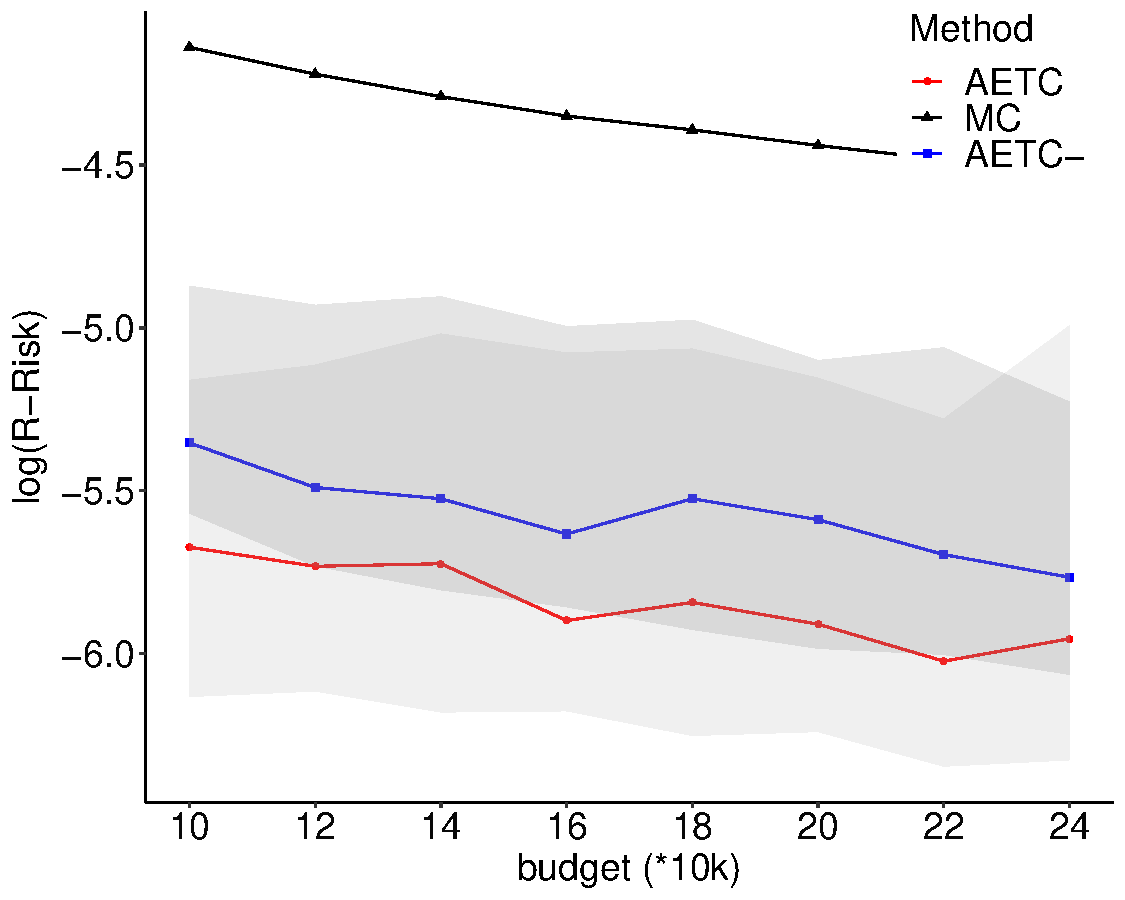
\includegraphics[width=7 cm]{mc2.pdf}
  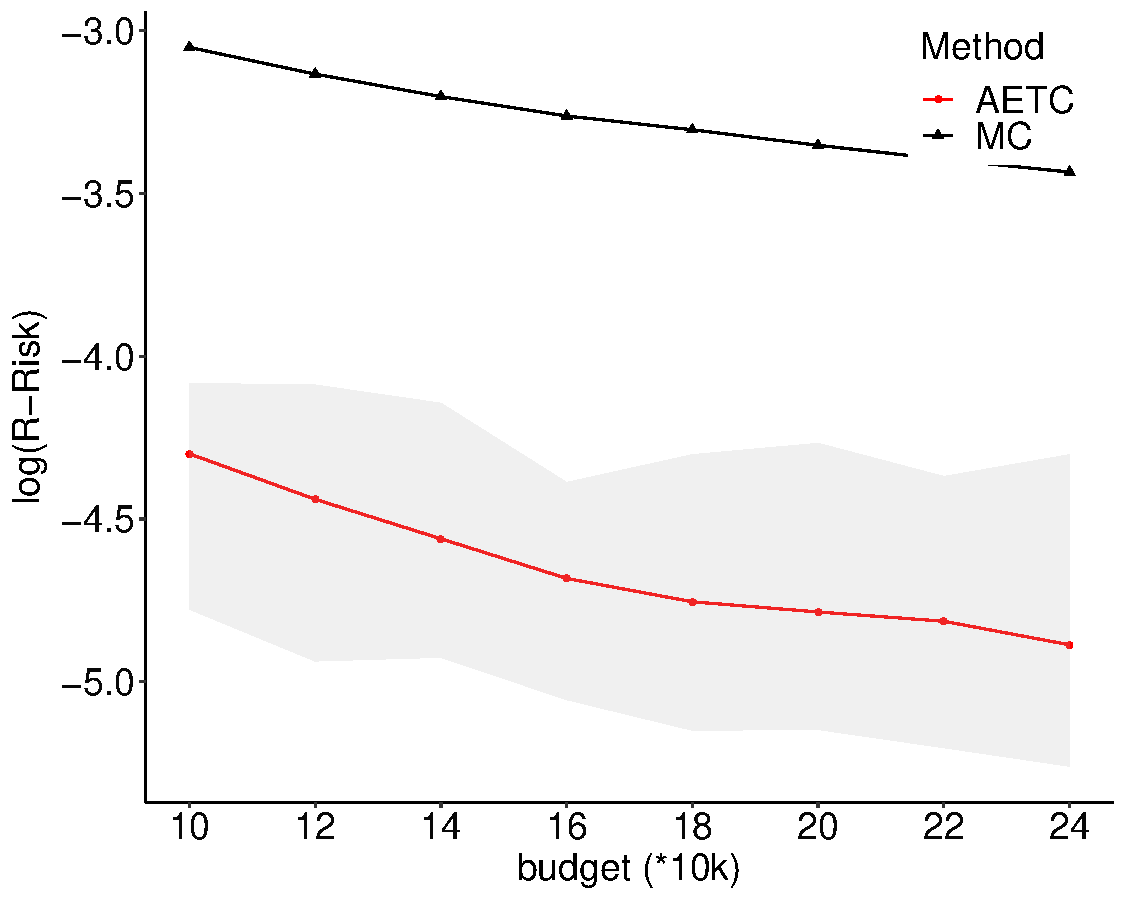
\includegraphics[width=7 cm]{mc.pdf}
  \caption{The left plot depicts the ($\log_{10}$) $Q$-risk of the AETC-LRMC estimator and the Monte Carlo estimator as budget increases from $100000$ to $240000$. The weight matrix $Q$ is taken as the identity matrix. The high-fidelity model output is taken as the value of a component whose index is randomly chosen and fixed thereafter. The correlations between the high-fidelity model and low-fidelity models (arranged in increasing order) are $0.229, 0.179, 0.112, 0.0113, -0.200$ and $-0.985$. In this case, the cheapest model has the highest correlation with the true model, which clearly violates the hierarchical structure. The AETC- is obtained by applying the AETC to the dataset without the last low-fidelity model. Particularly, we want to test if models having low correlations with the truth can be combined to make a good estimate. The right plot is the same comparison but the high-fidelity model corresponds to a $10$-dimensional vector response. }
  \label{fig:mcmc}
\end{figure}


\printbibliography

\end{document}